\documentclass[12pt,oneside]{uhthesis}
\usepackage{subfigure}
\usepackage[ruled,lined,linesnumbered,titlenumbered,algochapter,spanish,onelanguage]{algorithm2e}
\usepackage{amsmath}
\usepackage{amssymb}
\usepackage{amsbsy}
\usepackage{caption,booktabs}
\captionsetup{ justification = centering }
%\usepackage{mathpazo}
\usepackage{float}
\setlength{\marginparwidth}{2cm}
\usepackage{todonotes}
\usepackage{listings}
\usepackage{xcolor}
\usepackage{multicol}
\usepackage{graphicx}
\floatstyle{plaintop}
\restylefloat{table}
\addbibresource{Bibliography.bib}
% \setlength{\parskip}{\baselineskip}%
\renewcommand{\tablename}{Tabla}
\renewcommand{\listalgorithmcfname}{Índice de Algoritmos}
%\dontprintsemicolon
\SetAlgoNoEnd

\definecolor{codegreen}{rgb}{0,0.6,0}
\definecolor{codegray}{rgb}{0.5,0.5,0.5}
\definecolor{codepurple}{rgb}{0.58,0,0.82}
\definecolor{backcolour}{rgb}{0.95,0.95,0.92}

\lstdefinestyle{mystyle}{
    backgroundcolor=\color{backcolour},   
    commentstyle=\color{codegreen},
    keywordstyle=\color{purple},
    numberstyle=\tiny\color{codegray},
    stringstyle=\color{codepurple},
    basicstyle=\ttfamily\footnotesize,
    breakatwhitespace=false,         
    breaklines=true,                 
    captionpos=b,                    
    keepspaces=true,                 
    numbers=left,                    
    numbersep=5pt,                  
    showspaces=false,                
    showstringspaces=false,
    showtabs=false,                  
    tabsize=4
}

\lstset{style=mystyle}

\title{Visualización inteligente automática de datos}
\author{\\\vspace{0.25cm}Victor Manuel Cardentey Fundora}
\advisor{\\\vspace{0.25cm}Dayany Alfaro Gonz\'alez\\\vspace{0.2cm}Yudivi\'an Almeida Cruz}
\degree{Licenciado en Ciencia de la Computación}
\faculty{Facultad de Matemática y Computación}
\date{Fecha\\\vspace{0.25cm}\href{https://github.com/username/repo}{github.com/username/repo}}
\logo{Graphics/uhlogo}
\makenomenclature

\renewcommand{\vec}[1]{\boldsymbol{#1}}
\newcommand{\diff}[1]{\ensuremath{\mathrm{d}#1}}
\newcommand{\me}[1]{\mathrm{e}^{#1}}
\newcommand{\pf}{\mathfrak{p}}
\newcommand{\qf}{\mathfrak{q}}
%\newcommand{\kf}{\mathfrak{k}}
\newcommand{\kt}{\mathtt{k}}
\newcommand{\mf}{\mathfrak{m}}
\newcommand{\hf}{\mathfrak{h}}
\newcommand{\fac}{\mathrm{fac}}
\newcommand{\maxx}[1]{\max\left\{ #1 \right\} }
\newcommand{\minn}[1]{\min\left\{ #1 \right\} }
\newcommand{\lldpcf}{1.25}
\newcommand{\nnorm}[1]{\left\lvert #1 \right\rvert }
\renewcommand{\lstlistingname}{Ejemplo de código}
\renewcommand{\lstlistlistingname}{Ejemplos de código}

\begin{document}

\frontmatter
\maketitle

\begin{dedication}
    A mi familia que con su amor, esfuerzo
    y apoyo me han hecho quien soy.\\

    A las personas que sin compartir
    sangre son mi familia.\\

    A Floppy.
\end{dedication}
\begin{acknowledgements}
    A mis padres, Graciela y Jos\'e Manuel, por criarme con
    todo el amor y esfuerzo del mundo a pesar de las dificultades.\\
    
    A mi hermano Jos\'e Manuel, por ser el mejor hermano
    que hubiese podido pedir.\\

    A mi t\'ia Vicky, por ser otra madre para m\'i.\\

    A mis abuelos, Gustavo, Noelia y Ada, por siempre velar por m\'i.\\
    
    A Alicia, Sandra, Osvaldo y los pitis, por abrirme las puertas de su casa
    y aceptarme como uno m\'as.\\

    A Gabriela, por acompa\~narme desde ni\~no.\\

    A Karla y Amanda, por todas esas noches de desvelo que pasamos juntos.\\

    A mis compa\~neros y profesores, por todos los conocimientos y momentos compartidos.\\

    A la profesora Lucina, por su confianza absoluta y palabras de apoyo.\\

    A mis tutores, Yudivi\'an y Dayany, por su confianza y gu\'ia.\\
    

\end{acknowledgements}
\begin{opinion}
    El estudiante Victor Manuel Cardentey Fundora desarroll\'o satisfactoriamente el trabajo de
    diploma titulado ``Visualizaci\'on Inteligente Autom\'atica de Datos''. En este trabajo el
    estudiante propuso un sistema para la recomendaci\'on de configuraciones gr\'aficas basada en el
    aprendizaje de m\'aquinas sobre grafos.

    Su propuesta se basa, en esencia, en la adaptaci\'on de m\'etodos transductivos de \textit{Knowledge Graph Embedding}
    al contexto de la recomendaci\'on de visualizaciones a trav\'es de aplicar la metaheur\'istica de universos paralelos. Para 
    mostrar la viabilidad de la propuesta, se realizaron un conjunto de experimentos a trav\'es de los cuales se evidencian las posibilidades
    de la propuesta as\'i como sus limitaciones.

    Para poder afrontar el trabajo, el estudiante tuvo que revisar la literatura cient\'ifica relacionada con la
    tem\'atica as\'i como soluciones existentes y bibliotecas de software que pudieran ser apropiadas para su utilizaci\'on.
    Todo ello con sentido cr\'itico, determinando las mejores aproximaciones y tambi\'en las dificultades que presentan.

    Todo el trabajo fue realizado por el estudiante con elevada constancia, capacidad de trabajo y habilidades, tanto de gesti\'on,
    como de desarrollo e investigaci\'on.
    Por estas razones pedimos que le sea otorgada al estudiante Victor Manuel Cardentey Fundora la m\'axima calificaci\'on posible
    y, de esta manera, pueda obtener el t\'itulo de Licenciado en Ciencia de la Computaci\'on.

    \begin{center}
        Dr. Yudivi\'an Almeida Cruz\\
        Facultad de Matem\'atica y Computaci\'on\\
        Universidad de La Habana\\
    \end{center}

    \begin{center}
        Lic. Dayany Alfaro Gonz\'alez\\
        Facultad de Matem\'atica y Computaci\'on\\
        Universidad de La Habana\\
    \end{center}
   
   
\end{opinion}
\begin{resumen}
	El Big Data ha revolucionado los campos de 
	la industria y la ciencia, siendo com\'un, hoy en d\'ia, el an\'alisis de
	conjuntos de datos de gran tama\~no y dimensi\'on para obtener informaci\'on
	que apoye la toma de decisiones.
	La visualizaci\'on de datos es uno de los m\'etodos m\'as utilizados
	dentro del an\'alisis de datos. Sin embargo, la construcci\'on de visualizaciones es un proceso complejo donde intervienen
	m\'ultiples criterios de dise\~no. Con el objetivo de facilitar el an\'alisis visual de grandes conjuntos
	de datos se han propuesto sistemas que construyen y sugieren visualizaciones
	de forma autom\'atica a los analistas de datos. En este trabajo se presenta
	una propuesta de sistema de recomendaci\'on de configuraciones gr\'aficas basado
	en el aprendizaje de m\'aquinas sobre grafos, se detallan los aspectos
	t\'ecnicos de la implementaci\'on de un prototipo y se eval\'ua, de forma
	experimental, la validez de la soluci\'on obtenida.
\end{resumen}

\begin{abstract}
	Currently, Big Data has revolutionized the fields of
industry and science, being common the analysis of large and 
high dimensional datasets to support decission making.
Data visualization is one of the most used methods
within data analysis, however, visualization design is a complex process involving
multiple design criteria and there are
disagreements even among experts. In order to facilitate the visual analysis of large datasets
there have been proposed systems that automatically build and suggest visualizations
 to data analysts. In this work it is presented
a proposal for a graphical configurations recommendation system based on
machine learning on graphs, the technical aspects of a prototype's implementation
are detailed, and the obtained solution is evaluated in an experimental setting.

\end{abstract}
\include{FrontMatter/Contents}

\mainmatter

\chapter*{Introducción}\label{chapter:introduction}

El ascenso de la era de la informaci\'on 
caracterizado por la r\'apida expansi\'on
de Internet y la adopci\'on generalizada de las computadoras
personales ha provocado que una gran variedad de datos sean producidos
en un volumen y velocidad cada vez mayores. Este fen\'omeno denominado
Big Data ha tenido un gran impacto en el desarrollo de distintas \'areas de la actividad humana como la ciencia y la industria, ya que mediante el procesamiento de estas enormes colecciones de datos se obtiene informaci\'on actualizada y relevante que permite tomar decisiones de forma r\'apida y segura. Debido a los beneficios potenciales que presenta el Big Data ha sido necesario el surgimiento y evoluci\'on de tecnolog\'ias y procesos que permitan su utilizaci\'on, siendo el an\'alisis de datos de los procesos m\'as relevantes dentro de este ecosistema dado que durante el mismo se realiza el descubrimiento de informaci\'on.

Dentro del an\'alisis de datos existen m\'ultiples enfoques y facetas, resultando de particular inter\'es el an\'alisis exploratorio el cual utiliza estad\'istica descriptiva y visualizaciones para descubrir las caracter\'isticas principales de un conjunto de datos permitiendo generar hip\'otesis. En la actualidad este enfoque requiere de especialistas del dominio con profundos conocimientos t\'ecnicos y supone un gasto considerable de tiempo y esfuerzo debido al tama\~no y dimensi\'on de los conjuntos de datos y la ausencia de herramientas que faciliten un an\'alisis visual m\'as r\'apido.
Las herramientas actuales de visualizaci\'on de datos como Excel, Tableau y Spotfire ofrecen facilidades para la especificaci\'on manual de visualizaciones, sin embargo, carecen de la capacidad de guiar al usuario a trav\'es del espacio de posibles visualizaciones que se pueden especificar por lo cual el usuario debe de buscar a ciegas en este espacio hasta encontrar alguna que sea relevante, siendo esto un procedimiento tedioso con numerosos intentos y errores. 

Estas limitaciones fueron recogidas y analizadas por Vartak et al. % Add the biblio reference here
(2016) definiendo y proponiendo como soluci\'on los sistemas de recomendaci\'on de visualizaciones (VizRec) % Change the format of VizRec to match the paper
los cuales tienen como objetivo construir y recomendar de forma autom\'atica visualizaciones que resalten patrones o tendencias de inter\'es, permitiendo un an\'alisis visual m\'as r\'apido. % quotes here?
Esta definici\'on depende del concepto humano de \textit{inter\'es} el cual es subjetivo por lo que dicho art\'iculo plantea cinco ejes (caracter\'isticas) para definir \textit{inter\'es} los cuales se denominaron \textit{ejes de recomendaci\'on}. A partir de la publicaci\'on de este art\'iculo se han realizado varias implementaciones de este tipo de sistemas resolviendo distintas combinaciones de los ejes mediante diferentes enfoques computacionales.

[Definir los ejes que se van a resolver en este trabajo y hablar de las limitaciones de las implementaciones que han intentado resolver esos ejes?]

[Explicar como mi propuesta solucionar\'ia estas limitaciones o mejorar\'ia algo de lo que se ha hecho]

[Hablar de LETO]

\addcontentsline{toc}{chapter}{Introducción}

\chapter{Estado del Arte}\label{chapter:state-of-the-art}

La necesidad de extraer conocimiento a partir de conjuntos de datos
de tama\~no y dimensi\'on cada vez mayores, unido a la complejidad del
proceso de an\'alisis de datos conducen a la necesidad de crear herramientas
de \textit{software} que ayuden a los analistas durante este proceso.
Una de las herramientas propuestas han sido los sistemas de recomendaci\'on de visualizaciones \cite{vartak2017towards}, 
estos sistemas tienen como objetivo descubrir informaci\'on relevante y presentarla visualmente
al usuario de forma autom\'atica. Debido a su complejidad existen l\'ineas de investigaci\'on
enfocadas a subproblemas de la recomendaci\'on de visualizaciones, siendo uno de ellos
la recomendaci\'on de configuraciones gr\'aficas.

En este cap\'itulo se realiza una exposici\'on de los m\'etodos computacionales para la representaci\'on 
de visualizaciones y se analizan las propuestas de diferentes sistemas orientados a la
recomendaci\'on de configuraciones visuales.


\section{Lenguajes de visualizaci\'on de datos}
Los lenguajes de visualizaci\'on de datos son utilizados para especificar
relaciones entre los datos a visualizar y los componentes gr\'aficos.

La mayor\'ia de lenguajes de visualizaci\'on se enfocan en brindar a los usuarios humanos
un marco para definir los datos de inter\'es y c\'omo deben ser visualizados [\cite*{li2018echarts}, \cite*{tableau}]. 
Estos est\'an compuestos por datos (registros y transformaciones), 
componentes gr\'aficos (marcas, leyendas, ejes, etc...) y
m\'etodos para definir una funci\'on de correspondencia entre ambos. Suelen clasificarse
de acuerdo a su expresividad en lenguajes de bajo nivel y lenguajes de alto nivel \cite{qin2020making}.

Otros sistemas se enfocaron en dar una definici\'on m\'as conveniente de procesar
por algoritmos basados en inteligencia artificial permitiendo definir espacios de b\'usqueda de
visualizaciones \cite{godfrey2016interactive}.


\subsection{Lenguajes de visualizaci\'on de datos de bajo nivel}
Los lenguajes de bajo nivel son aquellos en los que el usuario debe de especificar c\'omo asociar los
datos a cada componentes gr\'afico utilizado, permitiendo un alto nivel de personalizaci\'on y detalle en
las visualizaciones resultantes.

Los lenguajes de prop\'osito general pueden utilizarse como lenguaje de visualizaci\'on de bajo nivel
mediante la implementaci\'on de bibliotecas de visualizaci\'on. Algunas de las bibliotecas desarrolladas
con este prop\'osito han sido Prefuse \cite{heer2005prefuse} en Java y Matplotlib \cite{matplotlib} en Python,
estos lenguajes orientados a objetos modelan
los elementos gr\'aficos mediante clases las cuales implementan m\'etodos para definir el mapeo con los datos.

Otra alternativa ha sido el desarrollo de lenguajes
de dominio espec\'ifico (DSL por sus siglas en ingl\'es) dentro de lenguajes de alto nivel. Por ejemplo,
Protovis \cite{bostock2009protovis} es un DSL desarrollado en JavaScript 
el cual est\'a enfocado en brindar las mayores capacidades de personalizaci\'on para el usuario.

Varios de estos lenguajes han sido dise\~nados con el fin de ser un lenguaje independiente utilizado como est\'andar
de especificaci\'on de visualiaciones para permitir su uso entre varias plataformas. Este es el caso de
Vega \cite{vegaLang} y ReactiveVega \cite{satyanarayan2015reactive} los cuales permiten definir visualizaciones utilizando
un paradigma declarativo sin estar contenidos dentro de otro lenguaje y han sido utilizados por varias plataformas de
visualizaci\'on.

\subsection{Lenguajes de visualizaci\'on de datos de alto nivel}
Los lenguajes de alto nivel permiten abstraer al usuario de ciertos elementos dentro de la construcci\'on
de las visualizaciones mediante la utilizaci\'on de valores por defecto y la adici\'on de restricciones a sus capacidades. Estos pueden
estar implementados sobre lenguajes de bajo nivel y suelen ser m\'as f\'aciles de utilizar por los usuarios.
%[Figura \ref{fig: vega_vs_vega_lite}].

Muchos de estos lenguajes han surgido durante el desarrollo de plataformas
de an\'alisis de datos enfocadas a usuarios sin conocimientos en programaci\'on para mejorar la experiencia de uso. 
Plataformas como Echarts con lenguaje de nombre hom\'onimo \cite{li2018echarts} y Tableau la cual utiliza VizQL \cite{hanrahan2006vizql}
permiten a los usuarios especificar visualizaciones con una sintaxis simple y concisa.

Otros lenguajes han sido dise\~nados para facilitar el desarrollo de ecosistemas de
visualizaci\'on de datos en torno a ellos. Por ejemplo, Vega-Lite \cite{satyanarayan2016vega} es un lenguaje actualmente utilizado
por m\'ultiples plataformas de an\'alisis de datos y ha sido llevado a lenguajes como Python, Ruby y R mediante
la implementaci\'on de bibliotecas como Altair, Vega.rb y Elm-Vega respectivamente \cite{vegaEco}.

Igualmente se pueden econtrar implementaciones dentro de otros lenguajes como gg2plot implementado
directamente sobre el lenguaje R \cite{wickham2010layered}.

\subsection{Lenguajes basados en predicados l\'ogicos}

Los lenguajes de visualizaci\'on basados en predicados l\'ogicos surgen
con las primeras aproximaciones de los cient\'ificos al problema de visualizaci\'on autom\'atica de
datos. Estos lenguajes han sido utilizados para modelar los espacios de b\'usqueda que utilizan los algoritmos
enfocados a resolver este problema \cite{godfrey2016interactive}.

Este tipo de enfoques intentan representar el conocimiento humano existente \cite{bertin1983semiology} en el dise\~no
de visualizaciones a trav\'es de definir condiciones l\'ogicas las cuales pueden ser comprobadas de forma
secuencial mediante instrucciones \textit{if-then-else} [\cite*{mackinlay1986automating}, \cite*{mackinlay2007show}, \cite*{roth1994interactive}, \cite*{wongsuphasawat2015voyager}, \cite*{moritz2018draco}].


% \begin{figure}[h!]
%     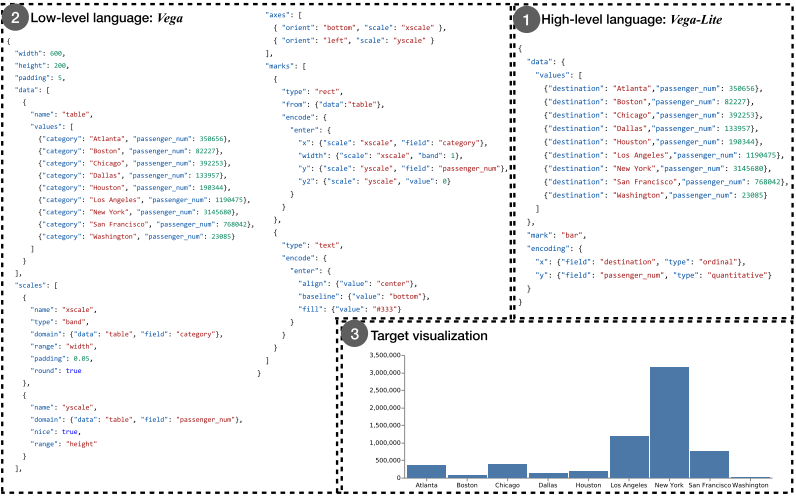
\includegraphics[width=\linewidth, height=70mm]{Graphics/vega_vs_vega_lite.png}
%     \caption{Comparaci\'on de complejidad entre los lenguajes Vega y Vega-Lite. 
%      (1) Ejemplo de c\'odigo utilizando el lenguaje Vega, (2) ejemplo de c\'odigo utilizando el lenguaje Vega-Lite,
%      (3) visualizaci\'on resultante en ambos casos.}
%     \label{fig: vega_vs_vega_lite}
% \end{figure}


\section{Sistemas de recomendaci\'on de configuraciones gr\'aficas}

La visualizaci\'on inteligente autom\'atica de datos tiene como objetivo
principal reducir el tiempo y esfuerzo necesitado para la exploraci\'on y
an\'alisis visual de los conjuntos de datos \cite{zeng2021we}. 

Las propuestas para
resolver dicho problema son denominados sistemas de recomendaci\'on de
visualizaciones (VizRec) y son un mecanismo de b\'usqueda en el espacio de visualizaciones
de acuerdo al inter\'es personalizado del usuario. A pesar de que el t\'ermino
VizRec fue recientemente concebido \cite{vartak2017towards}, el \'area, como tal, no es nueva.
Los primeros sistemas en generar visualizaciones de forma autom\'atica aparecer\'ian
a partir del a\~no 1986, manteniendose un alto inter\'es en el campo con el desarrollo
de nuevas soluciones y sistemas hasta la actualidad \cite{godfrey2016interactive}. 

Debido a la complejidad del problema de recomendaci\'on de visualizaciones muchos
sistemas optaron por intentar resolver un subproblema del mismo,
asumiendo la existencia de una especificaci\'on parcial de la visualizaci\'on donde el usuario haya seleccionado
los datos de inter\'es a visualizar. Esta versi\'on simplificada se plantea como el problema de la
recomendaci\'on autom\'atica de configuraciones gr\'aficas \cite{qin2020making}.

Generalmente los sistemas que resuelven este problema funcionan siguiendo un mismo procedimiento de dos pasos:
\begin{enumerate}
    \item Enumerar un conjunto de visualizaciones de inter\'es a partir de un espacio de visualizaciones.
    \item Utilizar una funci\'on de \textit{ranking} para ordenar el conjunto resultante.
\end{enumerate}

Actualmente existen dos enfoques principales para implementar este proceso: el enfoque basado en reglas
y el enfoque basado en aprendizaje de m\'aquinas. Los primeros han sido altamente estudiados dentro de la 
literatura debido que los primeros sistemas en aparecer fueron basados en reglas y la existencia
de numerosos trabajos acerca de pr\'acticas y heur\'isticas para dise\~no de visualizaciones facilitaba su desarrollo.
Por otro lado los enfoques basados en aprendizaje de m\'aquinas han tomado relevancia en los \'ultimos a\~nos con la aparici\'on
de varios prototipos \cite{zeng2021we}.

\subsection{Recomendaci\'on de configuraciones gr\'aficas basada en reglas} \label{subsection:rule-viz-rec}

Los sistemas de recomendaci\'on basados en reglas se caracterizan por el establecimiento
de condiciones bien definidas para la recomendaci\'on de visualizaciones. Estos sistemas
se pueden diferenciar de acuerdo al marco sobre el que se definen las condiciones: unos sistemas
se enfocan en representar el conocimiento humano en visualizaci\'on mediante programaci\'on l\'ogica y 
otros se centran en la utilizaci\'on de m\'etricas para la comparaci\'on de visualizaciones.

Los primeros sistemas en aparecer fueron basados en programaci\'on l\'ogica, estos propon\'ian lenguajes
l\'ogicos especiales para la representaci\'on de visualizaciones mediante un conjunto de reglas las cuales
se pod\'ian comprobar mediante instrucciones condicionales.

\textbf{Automatic Presentation Tool} (APT) \cite{mackinlay1986automating} fue el primer sistema de recomendaci\'on de visualizaciones.
En este enfoque las visualizaciones son definidas como oraciones de lenguajes
de visualizaci\'on de datos. Las consideraciones asociadas al dise\~no de visualizaciones
fueron implementadas como criterios de comparaci\'on para estos lenguajes. El criterio de expresividad
evaluaba cu\'anta informaci\'on (patrones, tendencias, anomal\'ias, etc...) era capaz de
transmitir el lenguaje. El criterio de efectividad evaluaba la utilizaci\'on de los
elementos gr\'aficos para facilitar la comprensi\'on de la informaci\'on transmitida.
El sistema generaba dise\~nos de forma autom\'atica utilizando composiciones algebraicas
de lenguajes de visualizaci\'on primitivos, luego los dise\~nos obtenidos eran recomendados de acuerdo
a los criterios de expresividad y efectividad.

\textbf{BOZ} \cite{casner1991task} recib\'ia como entrada una descripci\'on l\'ogica de
una tarea de an\'alisis a realizar sobre el conjunto de datos, esta descripci\'on estaba
basada en operadores l\'ogicos (representan operaciones sobre los datos) los cuales eran
sustuidos por operadores perceptuales (representan el uso de componentes gr\'aficos) mediante
el cumplimiento de reglas \textit{if-then-else}.


\textbf{SAGE} \cite{roth1994interactive} extendi\'o la soluci\'on propuesta por APT al permitir
la especificaci\'on total o parcial de las visualizaciones por los usuarios. Estas especificaciones
eran tratadas como directrices de dise\~no las cuales restring\'ian el espacio de b\'usqueda
analizado por el algoritmo que construye y compara las visualizaciones. El sistema pod\'ia construir
visualizaciones a partir de especificaciones sobre la informaci\'on relevante a mostrar o sobre
elementos de dise\~no gr\'afico.

\textbf{ShowMe} \cite{mackinlay2007show} es un sistema basado en APT. Este
trabajo introdujo el lenguaje de visualizaci\'on de datos de alto nivel llamado VizQL \cite{hanrahan2006vizql} el cual permite
especificar de forma algebraica la estructura de los gr\'aficos y los datos utilizados para generarlo.
Este sistema est\'a enfocado en la presentaci\'on visual y la experiencia de usuario por lo que las reglas y heur\'isticas implementadas
est\'an altamente influenciadas por los trabajos sobre dise\~no de visualizaciones y las m\'etricas utilizadas tienen como objetivo la expresividad de las visualizaciones. 

Por otro lado \textbf{Voyager} \cite{wongsuphasawat2015voyager} se enfoca en recomendar visualizaciones que muestren transformaciones 
sobre los datos seleccionados mediante
la utilizaci\'on de m\'etricas. Las configuraciones visuales son seleccionadas mediante la aplicaci\'on de reglas y heur\'isticas basadas en la literatura. 

\textbf{Draco} \cite{saket2018beyond} est\'a enfocado en el paradigma de la programaci\'on
basada en restricciones dentro de la programaci\'on declarativa. Un programa de restricciones 
es un conjunto de restricciones las cuales definen las relaciones entre un conjunto de variables cuyo
valor es desconocido. Este sistema introduce dos tipos de restricciones: las restricciones fuertes
las cuales deben de ser cumplidas por las soluciones del problema y las restricciones d\'ebiles las cuales
pueden violarse al costo de dicha soluci\'on sea penalizada. Estas restricciones restringen los posibles
valores de las variables y modelan la informaci\'on parcial sobre dichas inc\'ognitas. Las soluciones son
computadas como las de un problema de optimizaci\'on combinatoria sujeto a restricciones. Draco implementa
esta idea mediante una representaci\'on l\'ogica del lenguaje de visualizaci\'on Vega-Lite sobre la
cual un conjunto de expertos definen las restricciones y los pesos en caso de ser restricciones suaves.

\textbf{Learning Engine Through Ontologies} (LETO) \cite{estevez2019demo}, un marco de trabajo para el descubrimiento
de conocimiento mediante la creaci\'on y composici\'on de ontolog\'ias 
representadas utilizando grafos de conocimientos. Para la generaci\'on de configuraciones
se utiliz\'o un enfoque basado en reglas establecidas por los autores del sistema.

Los sistemas basados en m\'etricas se enfocan en utilizar medidas que caractericen la cantidad
de informaci\'on que transmite la visualizaci\'on. Estas m\'etricas provienen de distintas ramas
de la Matem\'atica y Computaci\'on. como .

Seo y col. \cite{seo2004rank} propone un sistema el cual recibe como especificaci\'on parcial el tipo de
gr\'afico (gr\'afico de barras, gr\'afico de puntos e histogramas), construye todos los posibles
gr\'aficos del tipo seleccionada y luego realiza un \textit{ranking} de acuerdo al valor de una m\'etrica seleccionada las
cuales eran espec\'ificas para cada tipo de gr\'afico. Por ejemplo, los histogramas utilizan m\'etricas enfocadas en propiedades
de la distribuci\'on de los datos mientras los gr\'aficos de puntos utilizaban la correlaci\'on, clusterizaci\'on y regresi\'on.

\textbf{SeeDB} \cite{vartak2014seedb} es un sistema el cual intenta maximizar el inter\'es del usario
al utilizar como referencia visualizaciones generadas o seleccionadas por el usuario
para recomendar aquellas visualizaciones que maximicen la desviaci\'on con los datos de la muestra.

\textbf{Foresight} \cite{demiralp2017foresight} realiza una clasificaci\'on de los tipos de gr\'aficos de
acuerdo al tipo de informaci\'on que pueden transmitir de acuerdo a consideraciones de dise\~no extra\'idas
de la literatura. Por ejemplo, los gr\'aficos de l\'inea suelen ser utilizados para mostrar correalaciones
mientras las gr\'aficas de caja permiten mostrar valores extremos. Esta clasificaci\'on permite reducir el tama\~no
del espacio de posibles visualizaciones mejorando la eficiencia del sistema con respecto a \cite{seo2004rank}.
Adem\'as incorpora cierta retroalimentaci\'on por
parte del usuario recomendando aquellos gr\'aficos que muestren el mismo tipo de informaci\'on que el gr\'afico
seleccionado por el usuario. Posteriormente \textbf{SpotLight} \cite{harris2021insight} extender\'ia este trabajo soportando
m\'as tipos de gr\'aficos y utilizando variadas m\'etricas de la Estad\'istica, Teor\'ia de la informaci\'on e Inteligencia artificial.

Este tipo de enfoque suele tener graves problemas de eficiencia debido a que se realizan exploraciones exhaustivas de los
espacios de b\'usqueda por lo que \cite{vartak2014seedb} propuso varias estrategias como podas, computaci\'on distribuida, etc...
Por otra parte los sistemas basados en reglas han presentado problemas para realizar la comparaci\'on entre visualizaciones debido
a la dificultad de realizar una definici\'on l\'ogica de criterios los cuales pueden ser subjetivos \cite{vartak2017towards}.

\textbf{DIVE} \cite{hu2018dive} propone un enfoque h\'ibrido que intenta resolver estos problemas combinando
la generaci\'on de visualizaciones mediante la composici\'on de lenguajes con el \textit{ranking} basado en m\'etricas. 

\subsection{Recomendaci\'on de Visualizaciones Basada en Aprendizaje de M\'aquinas}\label{subsection:ml-viz-rec}
En la actualidad existe un gran inter\'es en este tipo de enfoque apareciendo varias implementaciones
de estos sistemas con novedosas modelaciones del problema. 

\textbf{DeepEye} \cite{luo2018deepeye} divide el problema en dos subproblemas de aprendizaje de m\'aquinas. El primer subproblema es modelado
como un problema de clasificaci\'on binaria donde utilizando \'arboles de decisi\'on se aprende a etiquetar 
como \textit{buenas} o \textit{malas} las visualizaciones generadas para un conjunto de datos. 
El segundo subproblema consiste en un problema de \textit{Learning to Rank} (LTR) sobre el conjunto de visualizaciones. 
Para resolver este problema se cre\'o un corpus con pares de visualizaciones y el resultado de su comparaci\'on, luego esta funci\'on fue aproximada
mediante el algoritmo RankNet \cite{luo2018deepeye}. Para realizar las recomendaciones el sistema genera todas las posibles visualizaciones y enumera
aquellas clasificadas como \textit{buenas} por el primer modelo, finalmente este conjunto es ordenado de acuerdo a la funci\'on de \textit{ranking} aprendidad por
el segundo modelo. 

 

\textbf{Draco-Learn} \cite{moritz2018draco} es una extensi\'on de la propuesta del sistema Draco discutido en la
secci\'on \ref{subsection:rule-viz-rec}, una de las limitaciones principales de este sistema era la necesidad
de que expertos del dominio ajustaran los pesos de las restricciones suaves de forma manual. Este nuevo sistema
utiliza RankSVM para ajustar de forma autom\'atica los pesos de las restricciones utilizando un corpus de visualizaciones
generadas por expertos.


\textbf{Data2Vis} \cite{dibia2019data2vis} model\'o la recomendaci\'on de visualizaciones como un problema de
traducci\'on de lenguajes. Este sistema representa los datos de entrada mediante tuplas
relacionales definidas en el lenguaje JSON y su salida es un conjunto de sentencias
en el lenguaje de visualizaci\'on de datos Vega-Lite las cuales se corresponde con las
visualizaciones recomendadas. Esta traducci\'on se llev\'o a cabo utilizando m\'etodos
basados en redes neuronales recurrentes convencionales (RNN por sus siglas en ingl\'es).
Este tipo de redes neuronales son capaces de capturar el contexto de las oraciones debido
a sus estructuras de memoria y son muy utilizadas en sistemas de traducci\'on autom\'atica \cite{sutskever2014sequence}.

\textbf{VizML} \cite{hu2019vizml} propuso un enfoque basado en redes neuronales profundas modelando
el problema como una serie de problemas de clasificaci\'on para seleccionar opciones gr\'aficas. Por cada
configuraci\'on gr\'afica construyen un modelo que clasifica dicha configuraci\'on en sus respectivas opciones, por ejemplo,
la configuraci\'on \textit{eje} puede ser clasificada en \textit{x} o \textit{y}. De esta forma el sistema puede
seleccionar las opciones y construir las visualizaciones. Adem\'as
present\'o una nueva forma de representar conjuntos de datos mediante vectores de caracter\'isticas utilizando
m\'etricas estad\'isticas.

Quian y col. \cite{qian2020ml} desarrollaron una extensi\'on de la propuesta del sistema VizML.
Entre sus aportes est\'an la definici\'on de un marco de trabajo para la definici\'on del problema
de recomendaci\'on de visualizaciones como un problema de aprendizaje de m\'aquinas y la incorporaci\'on
de informaci\'on estructural sobre el conjunto de datos en la entrada del modelo.

\textbf{KG4Vis} \cite{li2021kg4vis} utiliz\'o
como referencia el trabajo realizado en VizML para modelar el problema de recomendaci\'on
mediante un grafo de conocimientos donde la selecci\'on de las configuraciones gr\'aficas se realiza
mediante la soluci\'on de problemas de predicci\'on de aristas.










\chapter{Recomendaci\'on de configuraciones gr\'aficas basada en ML sobre grafos}\label{chapter:ml-on-graphs}

Los grafos son estructuras utilizadas extensivamente en la Ciencia de la Computaci\'on y otras
ramas de la ciencia debido a su capacidad de modelar estructuras basadas
en objetos y las relaciones que se establecen entre estos. Fen\'omenos
tan distintos como redes sociales, estructuras moleculares, redes de prote\'inas y
preferencias de usuarios pueden ser modelados mediante grafos.

En la actualidad los grafos desempe\~nan un rol fundamental en el
aprendizaje de m\'aquinas. Se han dise\~nado muchos sistemas para hacer predicciones o descubrir patrones dentro
de datos representados con grafos. Por ejemplo, recomendar amigos en
redes sociales, clasificar el rol de las prote\'inas de acuerdo a sus interacciones
o predecir la ocurrencia de enlaces moleculares \cite{hamilton2017representation}.

En este cap\'itulo se presenta un marco de trabajo para modelar
el problema de recomendaci\'on de visualizaciones como un problema
de aprendizaje de m\'aquinas sobre grafos. En la secci\'on \ref{section:theoretical-framework}
se presenta el marco te\'orico necesario para la comprensi\'on del
resto del cap\'itulo y en la secci\'on \ref{section:graph-framework} se proponen
diferentes formas de modelaci\'on del problema. 


\section{Marco Te\'orico-Conceptual}\label{section:theoretical-framework}

En esta secci\'on se definen los conceptos principales de la teor\'ia de grafos
y se presentan las nociones b\'asicas del campo de aprendizaje de m\'aquinas
sobre grafos necesarias para el correcto entendimiento del marco de trabajo propuesto.

\subsection{Teor\'ia de grafos}

La teor\'ia de grafos se centra en el estudio de un modelo
matem\'atico propuesto por el matem\'atico Leonhard Euler en el
a\~no 1736 denominado grafo \cite{estrada2012structure}.

\begin{definition}
    Un \textbf{grafo} es un par formado por dos conjuntos $G = (V,E)$, 
    donde $v \in V$ representa un v\'ertice (o nodo) del grafo y $E$ es un conjunto
    de pares no ordenados de elementos de $V$ a los cuales se les llama aristas. $G$ est\'a
    asociado con una funci\'on de tipado de v\'ertices $f_v: V \to \mathcal{T}^v$ y 
    una funci\'on de tipado de aristas $f_e : E \to \mathcal{T}^e$. 
\end{definition}

% \begin{definition}
%     Un \textbf{grafo ponderado} es un grafo $G = (V,E)$ tal que existe una funci\'on
%     $w : E \to \mathbb{R}$ la cual para todo par de v\'ertices $v_i, v_j \in V$  asigna un
%     peso $w_{ij}$.
% \end{definition}

% \begin{definition}
%     Un \textbf{grafo homog\'eneo} $G_{homo}$ es un grafo tal 
%     que $|\mathcal{T}^v| = |\mathcal{T}^e| = 1$. Todos los v\'ertices pertenecen
%     a un mismo tipo y todas las aristas pertenecen a un mismo tipo.
% \end{definition}

\begin{definition}
    Un \textbf{grafo heterog\'eneo} $G_{hete}$ es un grafo tal 
    que $|\mathcal{T}^v| > 1 \vee |\mathcal{T}^e| > 1$. Existen v\'ertices y/o aristas
    de distinto tipo.
\end{definition}


Los grafos pueden ser representados computacionalmente de distintas formas, las formas
m\'as utilizadas son la matriz de adyacencia y las listas de adyacencia.


\begin{definition}
    Dado un grafo $G = (V,E)$ la matriz de adyacencia de $G$ es una matriz
    $M^{|V|\times|V|}$ tal que:
    
    $$
            M_{ij} =
        \left\{
            \begin{array}{ll}
                1  & \mbox{if } \{v_i, v_j\} \in E \\
                0 & \mbox{if } e.o.c
            \end{array}
        \right.
    $$

\end{definition}


\begin{definition}
    Sea un grafo $G = (V,E)$ la lista de adyacencia de un v\'ertice $v \in V$ es el conjunto
    $\{ u \in V : \{v,u\} \in E \}$.
\end{definition}

Estas formas de representaci\'on de grafos han mostrado problemas de eficiencia
para la implementaci\'on de m\'etodos de an\'alisis de grafos, teniendo un
alto costo computacional y espacial. Por tanto una de las principales l\'ineas de
investigaci\'on se dedica a la investigaci\'on de representaciones eficientes de grafos,
dentro de esta l\'inea surge el problema de \textit{graph embedding} el cual se enfoca en representar
grafos mediante vectores.

\begin{definition}
    El \textbf{problema de graph embedding} consiste en dado un grafo
    $G = (V,E)$ y un entero $k$, tal que $k \ll |V|$, representar el
    grafo $G$ en un espacio $k$-dimensional en el cual se deben de preservar
    las propiedades de dicho grafo.
\end{definition}

\subsection{Aprendizaje de m\'aquinas sobre grafos}
Los problemas de aprendizaje de m\'aquinas sobre grafos suelen ser 
clasificados en cuatro tipo de problemas:

\begin{itemize}
    \item \textbf{Clasificaci\'on de v\'ertices: } El objetivo de este problema es dado un grafo $G = (V,E)$
    predecir las etiquetas $l_u$ (de tipo, categor\'ia o atributo) asociadas
    a los v\'ertices $u \in V$, utilizando las etiquetas de un conjunto de nodos de entrenamiento $V_{train} \subset V$.
    \item \textbf{Predicci\'on de aristas: } El objetivo de este problema es dado un conjunto de
    v\'ertices $V$ y un conjunto incompleto de aristas $E_{train} \subset E$ inferir el conjunto
    de aristas faltantes $ E \setminus E_{train}$.
    \item \textbf{Detecci\'on de comunidades: } El problema de detecci\'on de comunidades es el an\'alogo
    en aprendizaje de m\'aquinas sobre grafos a los problemas de clusterizaci\'on, con el objetivo de
    detectar estructuras de comunidades dado como entrada un grafo $G = (V,E)$.
    \item \textbf{Clasificaci\'on, regresi\'on y clusterizaci\'on de grafos: } La clasificaci\'on y regresi\'on de grafos son problemas
    an\'alogos a los problemas tradicionales de aprendizaje de m\'aquina supervisado donde se tienen como entrada un conjunto de
    datos de entrada $X$ (en este caso grafos), un conjunto de datos de salida $Y$ y debe de aproximarse la funci\'on $h(X) = Y$. Igualmente
    el problema de clusterizaci\'on de grafos es an\'alogo al problema de aprendizaje no supervisado tradicional. 
\end{itemize}

Para resolver estos problemas los primeros enfoques utilizaban estad\'isticas
descriptivas sobre grafos, funciones de kernel o medidas para caracterizar las
estructuras de vecindad de los v\'ertices. Sin embargo, estos enfoques son limitados
dado este tipo de medidas son inflexibles y no pueden ser adaptadas durante el proceso
de aprendizaje. Un enfoque m\'as reciente
se basa en la soluci\'on del problema de \textit{graph embedding} mediante el aprendizaje
de funciones que permiten transformar v\'ertices, subgrafos o grafos enteros en
vectores del espacio $\mathbb{R}^K$. Este enfoque es
llamado \textit{Graph Representation Learning} (GRL) y ha permitido que
los grafos sean utilizados por m\'etodos tradicionales de aprendizaje de m\'aquinas.


\section{Modelaci\'on de la recomendaci\'on de configuraciones visuales mediante grafos}\label{section:graph-framework}

El marco de trabajo propuesto en esta investigaci\'on se compone de tres elementos:

\begin{itemize}
    \item La representaci\'on matem\'atica de una lenguaje de visualizaci\'on de datos que permite generar espacios de b\'usqueda.
    \item La representaci\'on de un conjunto de datos mediante grafos.
    \item La definici\'on de tareas de aprendizaje de m\'aquinas que permiten generar elementos del espacio de b\'usqueda.
\end{itemize}

\subsection{Definici\'on del espacio de b\'usqueda}

Para poder enumerar un conjunto de visualizaciones que recomendar
al usuario estos sistemas deben de ser capaces de definir un espacio
de posibles visualizaciones. Para ello se opt\'o por definir el
espacio de b\'usqueda como una selecci\'on de las opciones de configuraci\'on
graficas en un lenguaje de visualizaci\'on abstracto.

\begin{definition}[Lenguaje de Visualizaci\'on de Datos]
    Un lenguaje de visualizaci\'on de datos $\mathcal{C}$ es un
    conjunto de elementos $C_i \in \mathcal{C}$ los cuales son una
    abstracci\'on de las configuraciones gr\'aficas permitidas dentro
    del lenguaje. Cada elemento $C_i$ es un conjunto de elementos
    $\{ c_{i1}, c_{i2},..., c_{i|C_i|}\}$ los cuales representan las
    posibles opciones de la configuraci\'on.
\end{definition}

Un ejemplo de la especificaci\'on de un lenguaje mediante la definici\'on anterior
ser\'ia $\mathcal{C} = \{ \textbf{Eje} = \{ \textbf{x}, \textbf{y} \}, 
\textbf{Marca} = \{ \textbf{L\'inea}, \textbf{Punto}, \textbf{Barra} \} \}$

\begin{definition}[Espacio de visualizaciones]
    Sea un lenguaje de visualizaci\'on \\ $\mathcal{C} = \{ C_1, C_2, ..., C_n \}$
    el espacio de posibles visualizaciones generado por $\mathcal{C}$ es un
    conjunto $\mathcal{S} \subseteq C_1 \times C_2, \times ... \times C_n$.
\end{definition}

Esta definici\'on del espacio de b\'usqueda nos permite combinar configuraciones gr\'aficas y definir restricciones para
validar la construcci\'on visualizaci\'ones.

\subsection{Representaci\'on de conjuntos de datos mediante grafos}

Siendo este trabajo un primer paso en este enfoque se decidi\'o limitar su alcance
a las formas gr\'aficas traicionales como gr\'aficos de barras, l\'ineas, entre otros. Estas formas
gr\'aficas est\'an dise\~nadas para la representaci\'on de datos estructurados, el modelo de 
datos usualmente empleado para representar conjuntos de datos estructurados es el modelo relacional \cite{codd1970relational}.

La representaci\'on de conjuntos de datos en este marco de trabajo est\'a basada en dicho modelo permitiendo su
desarrollo sobre sistemas de bases de datos relacionales o sistemas de recomendaci\'on de visualizaciones que representen
la informaci\'on de forma relacional. Por tanto un conjunto de datos es una \textit{relaci\'on} cuya
representaci\'on visual es una tabla de filas y columnas.

En la actualidad el an\'alisis de datos es aplicado a numerosas
ramas del conocimiento humano por lo
que los dominios de diferentes conjuntos de datos pueden ser muy heterog\'eneos.
Incluso dentro de un mismo conjunto de datos los dominios pueden ser de
diferentes tipos (valores reales, cadenas, booleanos, etc...) y magnitudes.

Tomando en cuenta este problema se decidi\'o representar los conjuntos de datos
mediante la transformaci\'on de sus atributos a un espacio com\'un de dimensi\'on $K$.

\begin{definition}
    Se denota por $\sigma$  la funci\'on que realiza una transformaci\'on
    de un atributo $A$ de dominio arbitrario (y perteneciente a una relaci\'on
    arbitraria) a un espacio de dimensi\'on $K$.
    $$
        \sigma : A \to \mathbb{R}^K
    $$
\end{definition}

Esto permite representar un conjunto de datos $D$ de atributos $A_1, A_2, ..., A_n$ como un
conjunto de vectores $\{\sigma(A_1), \sigma(A_2), ..., \sigma(A_n)\}$ de dimensi\'on $K$.

Luego se procede a construir un grafo heterog\'eneo $G = (V,E)$ tal que $V$ es la uni\'on
de los distintos conjuntos de v\'ertices que representan las entidades del problema y $E$ es la uni\'on de los distintos
conjuntos de aristas que modelan las relaciones entre las entidades.

Se definieron los siguientes conjuntos de v\'ertices:
\begin{itemize}
    \item Conjunto de conjunto de datos $V_D$: este conjunto representa los conjuntos de datos.
    \item Conjunto de atributos $V_A$: este conjunto representa los atributos del conjunto de datos.
    \item Conjunto de propiedades $V_F$: este conjunto representa cada una de las $K$ dimensiones en las cuales son representados los atributos de los conjuntos de datos.
\end{itemize}

Se definieron las siguientes relaciones dadas por conjuntos de aristas:
\begin{itemize}
    \item \textit{Pertenecer} $E_{AD}$: este conjunto de aristas representa la relaci\'on de pertenencia entre un atributo y un conjunto de datos.
    \item \textit{Caracterizar} $E_{AF}$: este conjunto de aristas representa la relaci\'on de caracterizaci\'on entre una dimensi\'on del espacio de representaci\'on y los atributos.
\end{itemize}

\centering{
\begin{center}
    \begin{figure}[h!]
        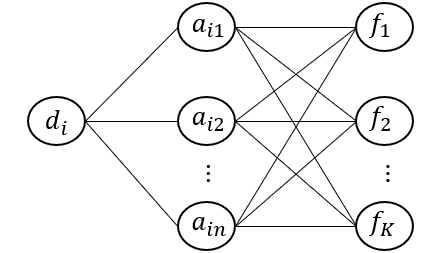
\includegraphics[width=90mm, height=50mm]{Graphics/basic_graph.png}
        \caption{Estructura de grafo propuesta}
        \label{fig: basic-graph}
    \end{figure}
\end{center}
}


\section{Tareas de aprendizaje de m\'aquinas}

El enfoque general para la resoluci\'on del problema es simular el proceso de
construcci\'on de un gr\'afico en un lenguaje de visualizaci\'on.

\begin{itemize}
    \item Seleccionar un atributo del conjunto de datos
    \item Seleccionar secuencialmente las opciones deseadas en la configuraci\'on gr\'afica de la visualizaci\'on: \begin{itemize}
        \item \bf Eje : x, y
        \item \bf Marca : barra, l\'inea, punto
        \item \bf Color : rojo, verde, azul
    \end{itemize}
\end{itemize}

Para generar el gr\'afico el usuario resuelve una serie de problemas de decisi\'on sobre las configuraciones gr\'aficas,
por este motivo dado un lenguaje de visualizaci\'on $\mathcal{C}$ con configuraciones gr\'aficas $C_1, C_2, ..., C_n$
definimos una tarea de aprendizaje de m\'aquinas por cada configuraci\'on $C_i$.

Es importante resaltar que se consideraron dos tipos de configuraciones gr\'aficas: las asociadas
a los atributos (p.e. eje, color, marca) y las asociadas al conjunto de datos (p.e. utilizaci\'on de leyendas y cuadr\'iculas).
La primeras dos tareas propuestas est\'an enfocadas a configuraciones de atributos y la tarea restante se utiliza para
las configuraciones de los conjuntos de datos.

\subsection{Problema de clasificaci\'on de v\'ertices}

Sean un grafo $G = (V,E)$ con $V = V_D \cup V_A \cup V_F$ y $E = E_{DA} \cup E_{AF}$, una configuraci\'on
gr\'afica $C$ y un conjunto $\mathcal{L}$ de etiquetas tal que existe una funci\'on biyectiva $f : \mathcal{L} \to C$.
Dado un conjunto de v\'ertices ${V_D}_l \subset V_D $ los cuales est\'an etiquetados el objetivo es aproximar la funci\'on
$h : V_D \to \mathcal{L}$ para inferir las
etiquetas para el conjunto $V_D \setminus {V_D}_l$ de v\'ertices no etiquetados. 

\subsection{Problema de predicci\'on de aristas}

Para este problema se modific\'o la arquitectura del grafo mostrada en la imagen \ref{fig: basic-graph}
a\~nadiendo el conjunto de v\'ertices $V_C$ el cual representa las posibles opciones de una configuraci\'on $C_i$ y
el conjunto de aristas $E_{AC}$ las cuales representan la utilizaci\'on una opci\'on para codificar un atributo.

\begin{figure}[h!]
    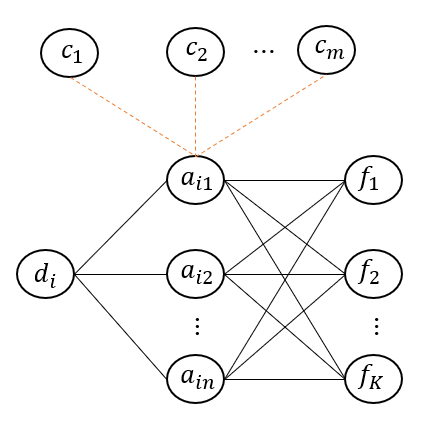
\includegraphics[width=85mm, height=65mm]{Graphics/link_pred_graph.png}
    \caption{Estructura de grafo propuesta para el problema de predicci\'on de aristas}
    \label{fig: link-pred-graph}
\end{figure}

Sean un grafo $G = (V,E)$ con $V = V_D \cup V_A \cup V_F \cup V_C$ y $E = E_{DA} \cup E_{AF} \cup E_{AC}$,
una configuraci\'on gr\'afica $C$ y $E_{AC}^*$ el conjunto de todas las posibles aristas entre los conjuntos de v\'ertices $V_A$ y $V_C$.
El objetivo es aproximar una funci\'on de probabilidad $p : E_{AC}^* \to [0,1]$ la cual indique la probabilidad de que una arista
entre un elemento $V_A$ y un elemento de $V_C$ pertenezca al grafo.

\subsection{Problema de clasificaci\'on de grafos}

Sean $C$ una configuraci\'on gr\'afica, $\mathcal{L}$ un conjunto de etiquetas y
una funci\'on biyectiva $f : \mathcal{L} \to C$. Dado un conjunto
de grafos etiquetados $\{(G_1, l_1), (G_2, l_2),..., (G_n, l_n)\}$, $l_i \in \mathcal{L} : 1 \leq i \leq n$ 
el objetivo es aproximar una funci\'on $h : \mathbb{G} \to \mathcal{L}$ donde
$\mathbb{G}$ es el espacio de todos los posibles grafos.



\chapter{Propuesta}\label{chapter:proposal}

El enfoque utilizado en este trabajo 

\section{M\'odulos del sistema}

El proceso comienza con la obtenci\'on de un conjunto de datos
ya existente del cual se quieren recomendar las configuraciones
gr\'aficas para visualizarlo. 

Los atributos de este conjunto de datos son transformados en vectores de caracter\'isticas
los cuales describen estos atributos mediante el c\'omputo de
m\'etricas estad\'isticas.

Luego los valores de las componentes de estos vectores son
discretizados y transformados en un grafo de conocimiento. Este
grafo es bipartito donde un conjunto de v\'ertices representa
los atributos del conjunto de datos y el otro conjunto representa
los posibles valores de las m\'etricas estad\'isticas utilizadas para
describirlos.

Luego este grafo es utilizado como la entrada de una red neuronal
artificial encargada de predecir la clase a la cual pertenencen los
v\'ertices del conjunto asociado a los atributos.

Definiendo una funci\'on de mapeo entre el espacio de clases existentes en este problema 
de clasificaci\'on y los posibles valores de las configuraciones gr\'aficas
disponibles se obtiene un sistema capaz de seleccionar de forma autom\'atica
configuraciones gr\'aficas para conjuntos de datos.


\begin{figure}[h!]
    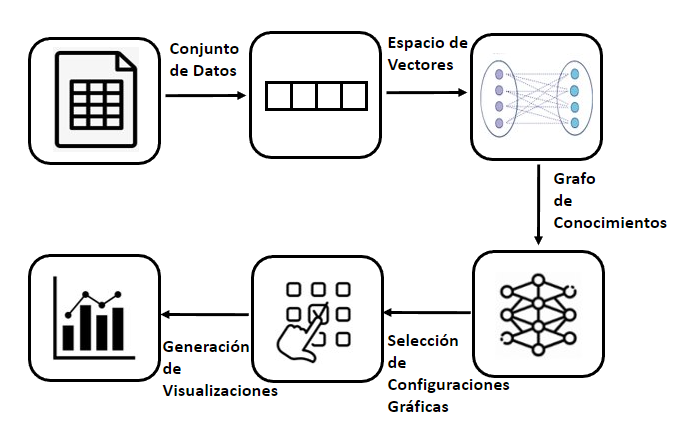
\includegraphics[width=\linewidth]{Graphics/simple_pipeline.png}
    \caption{Flujo de datos de la soluci\'on propuesta}
    \label{fig: flow_chart_sol}
\end{figure}


\subsection{M\'odulo de extraci\'on de caracter\'isticas}

El primer paso se encarga de transformar la entrada del sistema a un
espacio com\'un de $K$ dimensiones. Este proceso se realiza con el
objetivo reducir la heterogeneidad de los datos de entrada que utiliza
el modelo, debido a que los posibles conjuntos de datos a analizar
pueden provenir de distintos dominios del conocimiento humano (Medicina, Econom\'ia, etc...) \cite{vartak2017towards}.

La reducci\'on de dimensi\'on de un conjunto de datos se realiza mediante
la caracterizaci\'on de sus atributos. En este trabajo se decidi\'o caracterizar
los atributos mediante el uso de m\'etricas estad\'isticas el cual ha sido
un enfoque ampliamente usado en la literatura \cite{key2012vizdeck} \cite{vartak2014seedb} \cite{demiralp2017foresight} \cite{qian2020ml}.

Tambi\'en se toman en especial consideraci\'on problemas comunes
enmarcados dentro del an\'alisis de datos como la existencia de datos faltantes \cite{schafer2002missing}
y el soporte para distintos tipos de datos. Para ello se realiza un preprocesamiento
antes de calcular los estad\'isticos en el cual se realiza la inferencia de los tipos de datos utilizados
y la imputaci\'on de datos faltantes.

\subsection{M\'odulo de construcci\'on de grafos}

Despu\'es de obtener un conjunto de vectores de caracter\'isticas se realiza un proceso
de discretizaci\'on de las componentes de los vectores, esto tiene como objetivo aumentar
la densidad del espacio sobre el que se definen los atributos de los conjuntos de datos haciendo que 
el grafo resultante sea m\'as denso.
Cada componente es discretizada mediante la creaci\'on de intervalos que particionan el
rango de valores que puede tomar dicha componente. Para discretizar los
valores se utiliz\'o el algoritmo MDLP \cite{fayyad1993multi} el cual puede
inferir la cantidad de intervalos en que deben ser particionados los valores
bas\'andose en la distribuci\'on de los datos. Este algoritmo fue utilizado con
\'exito para esta tarea en \cite{li2021kg4vis}.

Luego se procede a construir el grafo de conocimiento, para ello se definen los conjuntos
de entidades $V_A$ que representa los atributos y $V_F$ el cual representa los posibles
rangos de valores para las distintas caracter\'isticas de los vectores. La relaci\'on entre
estos conjuntos se establece con el conjunto de aristas $E_{AF}$. Finalmente se
obtiene el grafo bipartito $G = (V_A \cup V_F, E_{AF})$.

En la literatura existen representaciones alternativas luego de la discretizaci\'on. \cite{qian2020ml} 
utiliza \textit{One Hot encoding} para representar la pertenencia
a intervalos de cada una de las m\'etricas de los atributos. Sin embargo, esto provoc\'o un 
aumento de la dimensi\'on de los vectores de caracter\'isticas lo cual conllev\'o
a emplear redes neuronales de mayores recursos.

\subsection{M\'odulo de modelos GRL}

\subsection{M\'odulo de generaci\'on de visualizaciones}
\chapter{Detalles de Implementación y Experimentos}\label{chapter:implementation}


\section{Herramientas y tecnolog\'ias utilizadas}

\subsection{Lenguaje de programaci\'on Python}

Python es un lenguaje de programaci\'on de alto nivel y de prop\'osito
general. Es interpretado, multi-paradigma, de tipado din\'amico y memoria
auto-manejada. Fue desarrollado por Guido Van Rossum en 1991 y la \'ultima
versi\'on al momento de realizarse este trabajo es la (incluirversion).
La mayor\'ia de las implementaciones incluyen un bucle \textit{Lectura-Evaluaci\'on-Impresi\'on}
(REPL por sus siglas en ingl\'es) funcionando como un int\'erprete de l\'ineas
de comandos, donde el usuario introduce las sentencias secuencialmente y recibe
inmediatamente los resultados.

En octubre de 2021 alcanz\'o el primer puesto en la lista de los lenguajes
de programaci\'on m\'as populares seg\'un el \'indice de la comunidad de
programaci\'on TIOBE 2021. Es utilizado por grandes organizaciones como
Google [PSF2021b], Yahoo[PSF2020], la NASA[PSF2021c], el CERN [CERN 2014],
Wikipedia, Amazon, Facebook, Instagram, Spotify, entre otros.

Es muy usado para el an\'alisis e ingenier\'ia de datos, aprendizaje
por computadoras e inteligencia artificial gracias a diversas bibliotecas
como NumPy, SciPy, Pandas, Matplotlib, Tensorflow, Keras, Pytorch, OpenCV y Networkx.
Para desarrollo web cuenta con marcos de trabajo como FastAPI, Flask y Django.
Adem\'as, se emplea en otros campos como la rob\'otica, el internet de las
cosas y la educaci\'on.
Para este trabajo se utiliz\'o la versi\'on 3.7 para lograr una retro-compatibilidad
alta.


\subsection{Pandas}
Pandas es una biblioteca de c\'odigo abierto del lenguaje Python orientada
a la manipulaci\'on y an\'alisis de datos. Su implmentaci\'on es
r\'apida, poderosa y f\'acil de usar lo que la ha convertido en
una herramienta muy popular entre los analistas de datos en dominios 
acad\'emicos y comerciales \cite{pandas2022}.
Esta biblioteca provee objetos para la manipulaci\'on r\'apida
y eficiente de conjuntos de datos, es compatible con m\'ultiples formatos
de almacenamiento de datos e implementa operaciones optimizadas para
modificar conjuntos de datos.

En este modelo Pandas es utilizada para realizar inferencia de tipos
sobre los atributos de los conjuntos de datos y fue fundamental para
la creaci\'on de los conjuntos de entrenamiento del modelo.

\subsection{Numpy}
Numpy es una biblioteca de c\'odigo abierto para el lenguaje de
programaci\'on Python que permite crear vectores y matrices de gran
tama\~no y de muchas dimensiones. Adem\'as, incluye
funciones para operar con sus matrices y vectores de una forma
c\'omoda, siendo comparable a Matlab en ese sentido. Internamente
utiliza el lenguaje C para la implementaci\'on de las funciones, por
lo que brinda un alto rendimiento \cite{harris2020array}.

Este trabajo utiliza las implementaciones eficiente de arreglos y m\'etodos estad\'isticos
de esta biblioteca dentro del proceso de extracci\'on de vectores de caracter\'isticas.

\subsection{SciPy}
SciPy es una biblioteca de c\'odigo abierto para el lenguaje de
programaci\'on Python la cual est\'a enfocada en proveer algoritmos
para problemas de optimizaci\'on, integraci\'on, interpolaci\'on,
c\'alculo de valores propios, ecuaciones algebraicas, ecuaciones diferenciales,
estad\'isticas entre otros. Gracias a la utilizaci\'on de estructuras
especializadas para el c\'omputo sobre arreglos y sus implementaciones
altamente eficientes escritas en lenguajes de bajo nivel como Fortran, C y C++
permite resolver problemas complejos en utilizando una sintaxis de alto nivel a la
vez que r\'apida y eficiente \cite{2020SciPy-NMeth}.

SciPy es utilizada dentro del modelo durante la extracci\'on de vectores
de caracter\'isticas para realizar el c\'omputo de m\'etricas estad\'isticas complejas.

\subsection{Scikit-Learn}
Scikit-Learn es una biblioteca de aprendizaje de m\'aquinas de c\'odigo abierto para el
lenguaje de programaci\'on Python. Presenta una gran colecci\'on de modelos
para la resoluci\'on de problemas enmarcados dentro del paradigma de aprendizaje de m\'aquinas.
En la actualidad incluye modelos para problemas de clasificaci\'on, regresi\'on, 
clusterizaci\'on, reducci\'on de dimensionalidad y optimizaci\'on de modelos \cite{scikit-learn}.

Varios modelos utilizados como punto de referencia para comparar los resultados
de los experimentos realizados han sido provistos por esta biblioteca, adem\'as se han
empleado sus m\'etodos de preprocesamiento para la preparaci\'on del corpus.

\subsection{Tensorflow y Keras}
Tensorflow es una plataforma de c\'odigo abierto desarrollada por Google para
aprendizaje por computadoras de extremo a extremo. Proporciona interfaces para
C++, Haskell, Java, Go, Rust y Python de forma oficial, adem\'as de interfaces de
terceros para C\#, Julia, R y Scala. Su implementaci\'on permite ejecutarse
eficientemente tanto sobre CPU como GPU y TPU \cite{tensorflow2015-whitepaper}.

Keras es una interfaz de alto nivel de Tensorflow que permite resolver problemas
de aprendizaje autom\'atico con un enfoque en el aprendizaje profundo de una forma
accesible y altamente productiva \cite{chollet2015keras}.

Tensoflow y Keras fueron utilizados para la implementaci\'on y entrenamiento 
del modelo de clasificaci\'on de nodos y en el modelo de clasificaci\'on utilizado
como punto de referencia.

\subsection{Google Colaboratory}
Es un servicio gratuito de Google que permite escribir y ejecutar
c\'odigo arbitrario de Python sobre recursos computacionales como GPU y TPU en
el navegador. Esta plataforma ofrece un entorno de trabajo de Python con buenos recursos computacionales,
bibliotecas y herramientas de aprendizaje autom\'atico pre-instaladas de forma
gratuita (tambi\'en se ofrece la posibilidad de aumentar los recursos computaciones del entorno mediante una suscripci\'on de pago).
Basada en Jupyter Notebook brinda en su plan gratuito 13 GB de RAM, 110GB de almacenamiento (extensible mediante la utilizaci\'on de Google Drive) y
la posibilidad de utilizar tanto CPU como GPU y TPU \cite{google2014colab}.

Este servicio fue utilizado para la creaci\'on del corpus, entrenamiento y evaluaci\'on
del modelo.









\backmatter

\begin{conclusions}
    El objetivo fundamental de este trabajo fue realizar una primera
    aproximaci\'on a la recomendaci\'on de configuraciones
    gr\'aficas mediante aprendizaje de m\'aquinas.
   
    A partir de la profundizaci\'on en el estado del arte de la representaci\'on
    computacional de visualizaciones y la recomendaci\'on de configuraciones gr\'aficas, se desarroll\'o un marco
    de trabajo abstracto para modelar la recomendaci\'on de configuraciones gr\'aficas,
    mediante enfoques de aprendizaje de m\'aquinas sobre grafos. Se concibi\'o
    una propuesta de sistema basado en el marco de trabajo propuesto, sobre cuya base se implement\'o un prototipo funcional.

    La adaptaci\'on de m\'etodos transductivos de \textit{knowledge graph embedding} 
    al contexto de la recomendaci\'on de visualizaciones, a
    trav\'es de la metaheur\'istica de universos paralelos, constituye el 
    aporte de este trabajo al campo de la visualizaci\'on inteligente autom\'atica de datos.
    
    Se ejecutaron experimentos que permitieron establecer
    la validez de la propuesta realizada mediante la evaluaci\'on del prototipo y
    se plante\'o un conjunto de factores que pudieran influir en los resultados
    del sistema. 
\end{conclusions}

\begin{recomendations}
    A partir de los desaf\'ios computacionales encontrados, as\'i como de los
    resultados obtenidos por el sistema desarrollado, se identifican nuevas l\'ineas
    de investigaci\'on que permitan mejorar la efectividad de los sistemas de
    recomendaci\'on de configuraciones gr\'aficas.

    \begin{itemize}
        \item La creaci\'on de corpus de dominios espec\'ificos que permitan
        evaluar el efecto de la heterogeneidad de los dominios sobre los sistemas
        de recomendaci\'on de visualizaciones.
        \item Los modelos implementados utilizan peque\~nos subgrafos del grafo de
        entrenamiento para realizar las predicciones, por lo que ser\'ia posible
        almacenar el grafo de entrenamiento en almacenamiento externo. Para esto se propone la
        implementaci\'on del sistema utilizando bases de datos orientadas a grafos.
        \item Incluir relaciones entre atributos mediante funciones multivariable utilizadas por sistemas 
        basados en reglas.
        \item Realizar estudios sobre las capacidades del sistema para incorporar preferencias de usuario
        mediante la adici\'on din\'amica de entidades y relaciones al grafo de entrenamiento.
    \end{itemize}


\end{recomendations}

\include{BackMatter/Bibliography}

\end{document}